\section{时钟同步}

分布式编辑-编译工作流示例。例如：2144, < 2143。调用编译器则 make 不会重新编译，因为缺乏时间同步导致文件时间戳不匹配。

物理时钟。有时我们只需要精确的时间，而不仅仅是顺序。基于协调世界时(UTC)的时间信号，可通过短波/长波无线授时台、BERTIE SRS (GNSS)、RISNTTDRLY/(NTP/PTP) HRS 等方式向用户提供授时服务。

铯133原子无干扰的基态超精细能级间。(国际计量大会1967)。为什么跃迁对应辐射的9192631770个周期。

时间同步困难：
\begin{itemize}
\item 硬件时钟本身的不精确性。
\item 网络延迟，如消息延迟会使服务器应答过时。
\end{itemize}

\subsubsection{时钟同步：偏移与漂移}
时钟偏移：两个时钟值之间的相对差异。
时钟漂移：本地时钟相对‘完美参考时钟’的时间偏差现象。
时钟漂移率：本地时钟相对‘完美参考时钟’在单位时间内产生的时间偏差量。

\paragraph{Cristian's Algorithm 概述}
\begin{enumerate}
\item 客户端发送请求数据包，用其本地时钟打上时间戳 $T_1$。
\item 服务器用其本地时钟记录收到请求的时间 $T_2$。
\item 服务器发送响应数据包，包含其本地时钟 $T_3$ 和 $T_h$。
\item 客户端用其本地时钟记录收到服务器响应的时间 $T_4$。
\end{enumerate}

\paragraph{Cristian's Algorithm: 偏移量计算}
客户端采样往返时间 $\delta$：$\delta = (T_4 - T_1) - (T_3 - T_2)$。但客户端知道 $\delta$，不知道请求延迟 $req$ 和响应延迟 $resp$。假设 $req = resp = \delta/2$，则偏移量 $\theta = T_3 + \delta/2 - T_4$。

\begin{figure}[htbp]
\centering
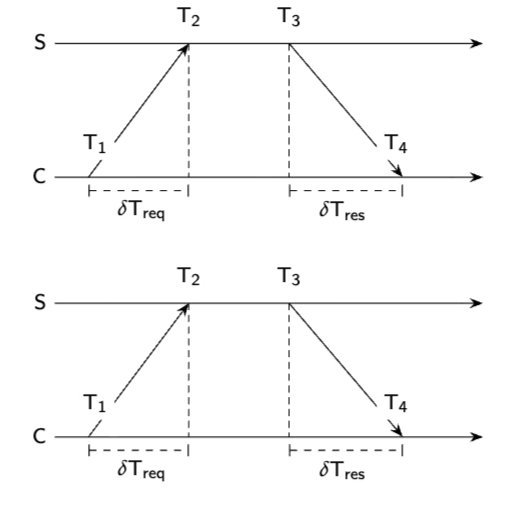
\includegraphics[width=0.8\textwidth]{figures/ch4/ch4_cristian_algorithm.png}
\caption{Cristian's Algorithm 往返时间计算示意}
\end{figure}

\begin{figure}[htbp]
\centering
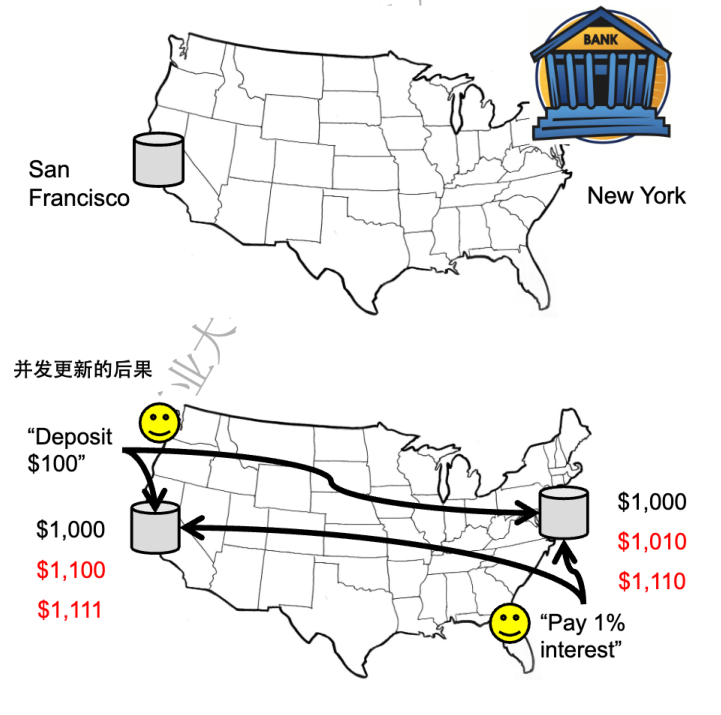
\includegraphics[width=0.8\textwidth]{figures/ch4/ch4_replica_inconsistency.png}
\caption{无协调下副本不一致示意}
\end{figure}

在无协调情形下，可能导致不一致的副本！更新应在每个副本上以相同的顺序执行。

\subsection{逻辑时钟}

\subsubsection{Lamport 逻辑时钟}

逻辑时钟。1978年Leslie Lamport的里程碑论文。洞察：只有事件顺序才是重要的，忽略精确的时间。捕获事件之间的“happens before”关系（$\to$ 关系）。通常重要的不是事件确切的时间，而是事件的发生顺序。

定义（$\to$）：
\begin{itemize}
\item 在同一进程中，如果事件 $a$ 发生在 $b$ 之前，则 $a \to b$。
\item 在不同进程中，如果 $a$ 是消息的发送，$b$ 是该消息的接收，则 $a \to b$。
\item 传递性：如果 $a \to b$ 且 $b \to c$，则 $a \to c$。
\end{itemize}

这在具有并发操作进程的系统中引入了事件偏序。
并发事件：并非所有事件都由 $\to$ 相关。$a$ 和 $b$ 不是由 $\to$ 相关，所以是并发的，记为 $a || b$。

\paragraph{Lamport 逻辑时钟}
问题：如何维护与“发生在之前”关系一致的系统行为的全局视图？
为每个事件 $e$ 附加一个时间戳 $LC(e)$，满足以下属性：
\begin{itemize}
\item P1: 如果 $a$ 和 $b$ 是同一进程中的两个事件，且 $a \to b$，则 $LC(a) < LC(b)$.
\item P2: 如果 $a$ 对应于消息 $m$ 的发送，$b$ 对应于该消息的接收，则 $LC(a) < LC(b)$.
\item P3: 对于所有事件 $a$ 和 $b$，如果 $a \to b$，则 $LC(a) < LC(b)$.
\end{itemize}

\paragraph{Lamport 逻辑时钟：实现规则}
每个进程 $P_i$ 维护一个本地计数器 $Clock_i$ 并调整：
\begin{enumerate}
\item 对于进程内发生的每个新事件，$Clock_i$ 增加1（属性P1）。
\item 每当进程 $P_i$ 发送消息 $m$ 时，消息时间戳 $LC(m) = Clock_i$（属性P2）。
\item 每当进程 $P_j$ 接收消息 $m$ 时，$P_j$ 将其本地计数器 $Clock_j$ 调整为 $\max(Clock_j, LC(m))$，然后在将 $m$ 传递给应用程序之前执行步骤1（属性P2）。
\end{enumerate}

两个事件仍可能同时发生。通过进程ID打破平局来避免这种情况。这里给大家板书演示一下。

\begin{figure}[htbp]
\centering
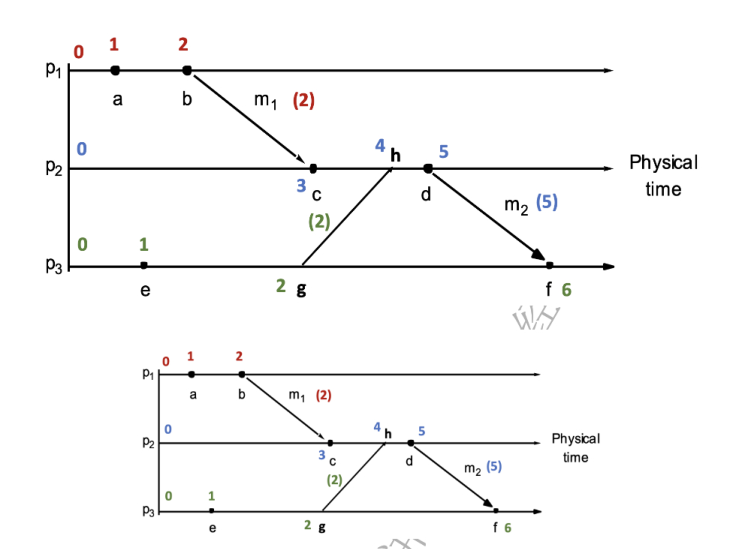
\includegraphics[width=0.8\textwidth]{figures/ch4/ch4_lamport_clock.png}
\caption{Lamport 逻辑时钟板书演示}
\end{figure}

一有两个副本。结果：在没有适当同步的情况下，副本\#1 为1111元，而副本\#2为1110元。

\subsubsection{全序多播推导（见板书）}

全序多播（ISIS）：
\begin{enumerate}
\item 发送阶段：发送者 $S$ 将一条消息 $M$ 多播给组内的所有接收者，这条消息被标记为“不可交付”（Undeliverable）。
\item 提议阶段（Bidding）：接收者 $P_i$ 收到消息 $M$ 后，查看每个本机最大序号记录（包括接收的和提议的），回复发送者一个“提议序号” $P_i = \max(\text{看到的最高序号}) + 1$。将 $M$ 放入一个优先级队列中，状态依然是“不可交付”，并暂时按提议序号排序。
\item 定标阶段（Selection）：发送者 $S$ 收集所有接收者返回的提议序号，从所有回复中选出最大值 $P_{max}$。这个 $P_{max}$ 就成为消息 $M$ 的最终序号。
\item 确认阶段（Commitment）：发送者 $S$ 再次多播一条确认消息，告诉所有人：“消息 $M$ 的最终序号是 $P_{max}$”。
\item 交付阶段（Delivery）：每个接收者收到确认消息后，将本地队列中消息 $M$ 的状态改为“可交付”，并按 $P_{max}$ 对队列重新排序。
\end{enumerate}

多站点复制的问题就这么容易的解决了吗？全序多播是否解决了多站点复制的问题？远非如此！我们的协议假设：无节点故障，无消息丢失，无消息损坏，All-to-all 通信不具扩展性，为消息延迟永远等待（性能差）。

\subsubsection{向量时钟}

Lamport时钟与因果关系。Lamport时钟时间戳可能无法捕获因果关系。即：不能保证如果 $LC(a) < LC(b)$，则 $a$ 因果上先于 $b$。给定 $LC(a)$ 和 $LC(z)$，我们想知道是否存在连接它们的事件链 $a \to \dots \to z$。

向量时钟：介绍。一个标量无法对多个进程中的事件进行排序，因而我们想将其扩展为一个向量。向量时钟 (Vector Clock) 是一个整数向量，分布式系统中每个进程都有一个。为事件 $e$ 标记 $VC(e) = [c_1, c_2, \dots, c_n]$。每个条目 $c_k$ 是进程 $k$ 中因果先于 $e$ 的事件计数。

\begin{figure}[htbp]
\centering
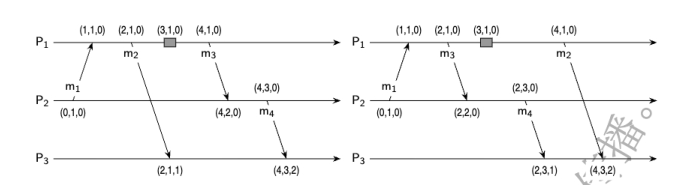
\includegraphics[width=0.8\textwidth]{figures/ch4/ch4_vector_clock.png}
\caption{向量时钟示例：多进程事件与向量时间戳}
\end{figure}

\paragraph{向量时钟：更新规则}
每个进程 $P_i$ 维护一个向量 $VC_i$：
\begin{itemize}
\item $VC_i[i]$ 是 $P_i$ 的本地逻辑时钟。
\item 如果 $VC_i[k] = k'$，则 $P_i$ 知道 $P_k$ 已经执行了 $k'$ 个事件。
\end{itemize}

初始时，所有向量都是 $[0,0,\dots,0]$。

两个更新规则：
\begin{enumerate}
\item 对于进程 $P_i$ 上的每个本地事件，执行前递增本地条目 $VC_i[i] := VC_i[i] + 1$。
\item 如果进程 $P_j$ 接收从 $P_i$ 发来的消息，并附带向量 $d = [d_1, d_2, \dots, d_n]$，则：
   \begin{itemize}
   \item 对每个 $k$，$VC_j[k] := \max(VC_j[k], d_k)$；然后 $P_j$ 递增自己的条目 $VC_j[j] := VC_j[j] + 1$。
   \end{itemize}
\end{enumerate}

交付给上层应用。

\paragraph{向量时钟：比较}
比较向量时间戳的规则：
\begin{itemize}
\item $VC(a) = VC(b)$ 当且仅当对所有 $k$, $VC(a)[k] = VC(b)[k]$，则 $a$ 和 $b$ 是同一事件。
\item $VC(a) < VC(b)$：对所有 $k$, $VC(a)[k] \le VC(b)[k]$，且存在 $k'$, $VC(a)[k'] < VC(b)[k']$，则 $a \to b$。
\item 并发性：如果存在 $i,j$，使得 $VC(a)[i] < VC(b)[i]$ 且 $VC(a)[j] > VC(b)[j]$，则 $a || b$。
\end{itemize}

\paragraph{比较Lamport时钟和向量时钟}
两个事件 $a$, $z$：
\begin{itemize}
\item Lamport时钟：$LC(a) < LC(z)$ 不能推导出 $a \to z$，即可能 $a \to z$ 或 $a || z$。
\item 向量时钟：$VC(a) < VC(z) \Rightarrow a \to z$。
\end{itemize}

拓展：向量时钟可以用来实现因果有序多播，即：确保仅当所有因果先于待交付消息的消息已被传递时才传递消息。例子：腾讯文档。

\paragraph{因果有序多播}
原则：如果消息A在逻辑上先于消息B产生，那么任何接收者都必须先处理A，再处理B。即保证所有存在happens-before关系的消息顺序。

实现方式：
\begin{itemize}
\item 发送端：当进程 $P_i$ 想要发送消息 $m$ 时：自增计数器 $VC_i[i] := VC_i[i] + 1$，不仅发送消息 $m$，还会把此时自己本地持有的整个向量 $[VC_i[1] \dots VC_i[N]]$ 附带在消息里。发送者在信封里塞了一张清单，告诉所有人：“这是我发的第 X 封信，在此之前，我已经收到了其他进程的这么多封信。”
\item 接收端：当进程 $P_j$ 收到来自 $P_i$ 的消息 $m$（附带有向量 $V$）时，它不会立即交付，而是先放在缓冲区，检查以下两个条件：
  \begin{enumerate}
  \item 消息序列连续性：$V[i] = VC_j[i] + 1$。这个消息必须是 $P_i$ 发出的“下一封”。
  \item 所有因果依赖都满足：对所有 $k \ne i$，$V[k] \le VC_j[k]$。即 $P_i$ 发出这封信之前，它所见过且来自其他所有进程的消息，$P_j$ 都已经接收并处理了。
  \end{enumerate}
\item 交付：当上述两个条件同时满足时：
  \begin{itemize}
  \item 提交：消息 $m$ 被正式交付给应用层（CO-deliver）。
  \item 更新状态：$VC_j[i] := V[i]$；对所有 $k$, $VC_j[k] := \max(VC_j[k], V[k])$。$P_j$ 记录下自己已经处理完 $P_i$ 的最新进展。
  \end{itemize}
\end{itemize}

全序多播是一种利用 Lamport 时钟实现分布式系统中事件全局排序的方法。全序多播协议需要仔细处理消息确认，以确保事件按正确顺序处理。尽管全序多播有用，但它假设了理想的网络和节点条件，且扩展性有限。

\begin{figure}[htbp]
\centering
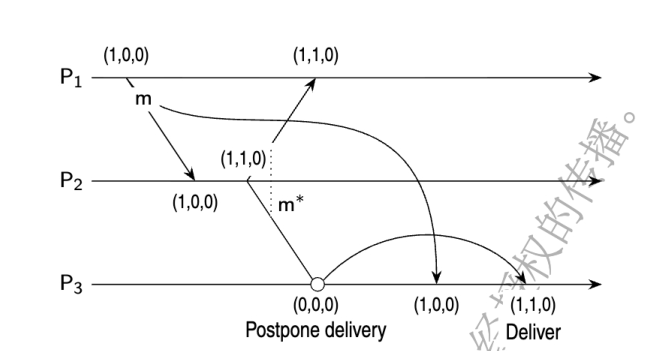
\includegraphics[width=0.8\textwidth]{figures/ch4/ch4_total_order_multicast.png}
\caption{全序多播协议流程}
\end{figure}

在分布式系统中可以对事件进行全序排序。根据构造，$a \to b$ 意味着 $LC(a) < LC(b)$ 一定成立。但命题的逆不成立：$LC(a) < LC(b)$ 不一定意味着 $a \to b$。注意不能使用Lamport时间戳来推断事件之间的因果关系。举例：Lamport时钟不能保证：如果 $LC(a) < LC(c)$，我们不能得出“$a$ 在因果上先于 $c$”。

逻辑时钟位于哪里？

示例应用：全序多播。
全序多播：所有消息都按相同的顺序传递给每个接收者。
复制数据库上的并发更新在各副本处以相同的Lamport时钟顺序执行。
例如：P1向账户添加100美元（初始值：1000美元）。
[图示：消息交付应用，复制数据库，物理时间轴...]
